\documentclass[class=book, crop=false, oneside]{standalone}
\usepackage[subpreambles=true]{standalone}

\usepackage{../../style}

\graphicspath{{./assets/images/}}
\newmintinline{asm}{}

% arara: pdflatex: { synctex: yes, shell: yes }
% arara: latexmk: { clean: partial }
\begin{document}
\chapter{Pipeline}

\section{Introduzione}
Nei capitolo precedenti è stato presentato lo schema base di un semplice processore che esegue un'operazione per ogni ciclo di clock, tuttavia questo metodo è molto svantaggioso in quanto il clock deve essere calcolato secondo la durata delle operazioni più lente, quindi se si implementano operazioni complesse questo rallenta di molto la velocità del processore, rendendo impossibile compiere ottimizzazioni \emph{aggressive} sulle operazioni più comuni.

In che modo è quindi possibile migliorare il rendimento della CPU?
Uno dei modi più semplici è quello di parallelizzare il lavoro, nello stesso modo con cui Henry Ford migliorò la produzione delle fabbriche del primo Novecento.

Il salto logico sta nel comprendere che mentre una componente A della CPU sta lavorando sull'operazione corrente un'altra componente B (precedente) può iniziare a svolgere l'operazione successiva; in tal modo si lo svolgimento delle operazioni non è più prettamente sequenziale ma diventa, in un certo senso, accavallato (lo svolgimento di un'operazione avviene nello stesso momento dello svolgimento di un'altra ma le due operazioni si trovano in fasi di completamento diverse).

Una misura del miglioramento che si introduce con metodi come il lavoro in parallelo è data dal trhoughput che è il numero di operazioni risolte per unità di tempo; in una catena di lavoro in parallelo composta da \(n\) stadi il miglioramento percentuale massimo ottenibile è \(n*100\), che è una percentuale assolutamente molto rilevante.

???Parliamo di lavatrici???

\subsection*{Pipeline}
Il concetto di Pipeline è esattamente quello di una catena di montaggio traslato nel campo delle operazioni di una CPU, ovvero Pipeline si dice di un'immplementazione della CPU che prevede lo svolgimento di iù operazioni in parallelo.

Tornando al nostro caro vecchio MIPS, ricordiamo brevemente quali sono le fasi dell'esecuzione di un'istruzione:
\begin{enumerate}[noitemsep]
	\item Fetch;
	\item Lettura registri e decodifica dell'istruzione;
	\item Esecuzione di un'operazione (di tipo R) o calcolo di un indirizzo;
	\item Accesso ad un operando nella memoria dati (nel caso di \opcode{lw} o \opcode{sw});
	\item Scrittura del risultato in un registro (\emph{writeback}).
\end{enumerate}
Quindi la pipeline che useremo per parallelizzare il lavoro della CPU possiederà 5 stadi.

\section{Un esempio}
Per comprendere meglio il concetto è presentato di seguito un esempio semplificato di pipeline, in cui le uniche operazioni possibili sono:
\begin{itemize}[nolistsep]
	\item \opcode{lw} e \opcode{sw} di accesso alla memoria;
	\item \opcode{and}, \opcode{or} e \opcode{slt} di tipo R;
	\item \opcode{beq} di tipo salto.
\end{itemize}
Naturalemnte i tempi necessari per il compimento di queste operazioni non sono uguali, è riportata quindi una tabella con annessi i tempi che (nel nostro esempio) servono per ogni categoria di operazione.

INCLUDI TABELLA QUI

Si nota che l'istruzione più lenta di tutte è la \texttt{load word}\footnote{Si noti che questa è l'unica istruzione che esegue effettivamente tutte le 5 fasi descritte in precedenza} e di conseguenza il tempo di clock viene definito in base ad essa.

Inoltre il tempo dedicato ad ogni singola fase del processo di esecuzioen è definito in base al tempo della fase con durata massima, ovvero nel nostro caso \unit[200]{ps}; questo implica che anche le fasi con durata inferiore verranno eseguite in un tempo di \unit[200]{ps} ed anche che la durata dell'esecuzione di una singola istruzione nella nostra pipeline è di \((tempo.singola.fase)*(numero.fasi)=200ps*5=1000ps\).

Osserviamo quindi un diagramma temporale per sequenza istruzioni in cui si confronta lo svolgimento di operazioni con il metodo standard e attraverso l'implementazione della pipeline.

INSERISCI DIAGRAMMA QUI


\subsection{Osservazioni}
La teoria ci dice che per avere una stima delle prestazioni della CPU una volta impleentata una pipeline si può usare la formula \[\text{Tempo tra due istruzioni con pipeline} = \frac{\text{Tempo tra due istruzioni senza pipeline}}{\text{Numero di stadi della pipeline}}\]

Quindi teoricamente questa formula nel nstro caso prevede un miglioramento delle prestazioni di un fattore 5, tuttavia si può notare che il tempo per eseguire 3 istruzioni passa da \unit[2400]{ps} a \unit[1400]{ps}, generando quindi un miglioramento di un fattore 1.7.

Le cause di questa discrepanza son principalmente due, in primis si deve sottolineare che per ottenere una prestazione 5 volte più alta il tempo di clock dovrebbe essere uguale a \(800/5=\) \unit[160]{ps}, mentre nella realtà non possiamo scendere sotto ai \unit[200]{ps} pichè ci sono delle fasi che hanno tale durata; in secondo luogo abbiamo considerato poche istruzioni, questo implica che non abbiamo fatto in tempo a distribuire il costo di "avvio" e di "terminazione" della pipeline (i due periodi in cui la pipeline non è completamente a regime), naturalmente il miglioramento si osserva meglio quando il numero di istruzioni è ben più alto del numero delle fasi della pipeline.

INSERIRE DUE CALCOLETTI???

\section{Vantaggi del RISC}
L'architettura di tipo RISC presenta dei vantaggi sostanziali per quanto riguarda il processo di \emph{pipelining}, sono riassunti nell'elenco sottostante.
\begin{itemize}
	\item Tutte le istruzioni hanno la stessa lunghezza. Questo facilita di molto il prelievo (sempre una word).
	\item I codici degli operandi sono in posizione fissa, questo permette di accedervi leggendo il registerfile in parallelo con la decodifica dell’istruzione.
	\item Gli operandi residenti in memoria sono possibili solo per \opcode{lw} e \opcode{sw}. Ciò permette di usare la ALU per il calcolo di indirizzi (cosa che non sarebbe possibile se dovessimo usare le ALU in due fasi della stessa istruzione, come è richiesto in ISA più complesse).
	\item  L’uso di accessi allineati fa sì che gli accessi in memoria avvengano sempre in un ciclo di trasferimento (impegnando un solo stadio della pipeline).
\end{itemize}

\section{Condizioni di Hazard}
In condizioni normali unapipeline permette di eseguire un'sstruzione per ciclo di clock, tuttavia questo non è sempre possibile, soprattutto quando si verificano delle determinate condizioni critiche dette \emph{hazard}.
Esistono diversi tipi di hazard:
\begin{itemize}
	\item Hazard strutturali;
	\item Hazard sui dati;
	\item Hazard sul controllo.
\end{itemize}
Osserviamo quindi come vengono a verificarsi queste condizioni critiche e quali sono le soluzioni più comuni adottate per risolverle.

\subsection{Hazard strtturale}
Una condizione di hazard strutturale è una condizione che si verifica qundo l'architettura dell’elaboratore rende impossibile l’esecuzione di alcune sequenze di istruzioni in pipeline.

Ad esempio, se io disponessi di un’unica memoria, non potrei nello stesso ciclo di clock, caricare istruzioni e memorizzare (o prelevare) operandi dalla memoria, ed è per questa ragione che esistono separatamente memoria dati e memoria istruzioni.

\subsection{Hazard sui dati}
Per spiegare questo hazard ricorriamo al seguente esempio di codice MIPS:
\begin{minted}{asm}
add $a0, $t0, $t1
sub $t2, $s0, $t3
\end{minted}
Nel momento di implementare questo codice tramite pipeline si noterebbe che \register{\$a0} viene salvato nella quinta fase di \opcode{add}, ma lo stesso registro è necessario nella seconda fase di \opcode{sub}, e quindi volendo implementare la pipeline si dovrebbe lasciare il processore in stallo per il tempo necessario per la memorizzazione di \register{\$a0}.
% che suscedi a questo comando register?

Esistono dei metodi per evitare questo spreco di tempo (ben tre fasi di attesa), il più semplice ma spesso anche il più funzionale prevede un rimescolamento delle istruzioni che riesce ad allontanare tra loro le due istruzioni quanto basta per far si che la prima termini in tempo per garantire la corretta esecuzione della seconda, tuttavia questa strada non è sempre percorribile.
Da ntare il fatto che questa è una delle operazioni che compilatori come il GCC compiono nella fase di trasuzione da linguaggio ad alto livello ad assembly.

Una soluzione ancora più efficiente è quella dell'\emph{operand forwarding}, detto anche propagazione o bypass, che prevede di rendere il contenuto del registro \register{\$a0} disponibile per l'operazione successva ancora prima che questo sia effettivamente salvato nel registro stesso, dato che quel valore sarà già noto dalla fase "execute".
Si osservi lo schema riportato qui sotto per una maggiore comprensione del meccanismo di propagazione.

INSERISCI IMMAGINE PROPAGAZIONE

\subsection{Hazard sul controllo}
Questo tipo di hazard riguarda nello specifico e operazioni di salto condizionato, che generano problemi in quanto prima di eseguirle del tutto non si può sapere quale sarà l'istruzione sucessiva, e se la pipeline è composta da tante fasi il tempo di attesa diventa assai svantaggioso.
Per il resto del capitolo consideriamo di avere un circuito molto sofisticato che ci permette di calcolare l’indirizzo di salto già al secondo stadio, tuttavia questo non basta poichè dobiamo lasciare la pipeline iin stallo per almeno una fase prima di sapere qual'è l'istruzione successiva.

Esistono tre? tipi di soluzione all'hazard sul controllo, sono riportate in seguito in ordine di complessità.
% non sarei proprio così sicuro che si possano sistemare così le cose in effetti
Il primo approccio prevede di risistemare l'ordine delle istruzioni come si farebbe per risolvere un hazard sui dati, che funziona ma non sempre è possibile.

Il secondo approccio viene chiamato \emph{untaken branch} che consiste nel considerare sempre che il salto non si verifichi e quindi far proseguire la pipeline nell'esecuzione delle operazioni regolarmente.

Una volta che la condizione del salto viene verificata se il salto non deve avvenire allora non c'è nessun problema e la pipeline può proseguire tranquillamente il suo lavoro, mentre in caso contrario si deve riristinare lo stato del processore al quello recedente l'istruzione del salto e far avvenire il salto stesso.
Questo implica la necessità di creare dei \emph{registri di backup} dove si va a salvare per l'appunto lo stato del processore ogni volta che si esegue il fetch di una operazione di salto condizionale.

IL terzo approccio è una versione più raffinata del secondo che prevede l'implementazione di una circuiteria di \emph{branch prediction}, che serve appunto per dare una stima della probabilità con cui avverrà il salto, questo permette di avere dei miglioramenti sull'efficienza del meccanismo \emph{untaken branch}.

Un circuito di \emph{branch prediction} calcola a runtime la probabilità con cui si verificherà un salto condizionale e può decidere se settare il comportamento standard come \emph{untaken branch} o come \emph{taken branch}, se ad esempio un programma prevede che un ciclo venga eseguito 1000 volte il circuito dopo qualche ripetizione setterà la risposta standard a \emph{taken branch} e quindi risparmierà molte fasi di "ripristino dello stato della CPU" dovute ad errori di predizione.

\subsection{Registri di backup}
Come detto in precedenza per meccanismi come l'\emph{untaken branch} e l'implementazione di \emph{branch prediction} si rendono necessari dei registri da utilizzare come backup nel caso la predizione effettuata si riveli errata, nell'immagine presente qui sotto si possono osservare questi tali registri, si noti che il nome dei registri viene dato a seconda delle fasi che separano (information fetch/information decode/execute...).
\begin{figure}[H]
	\centering
	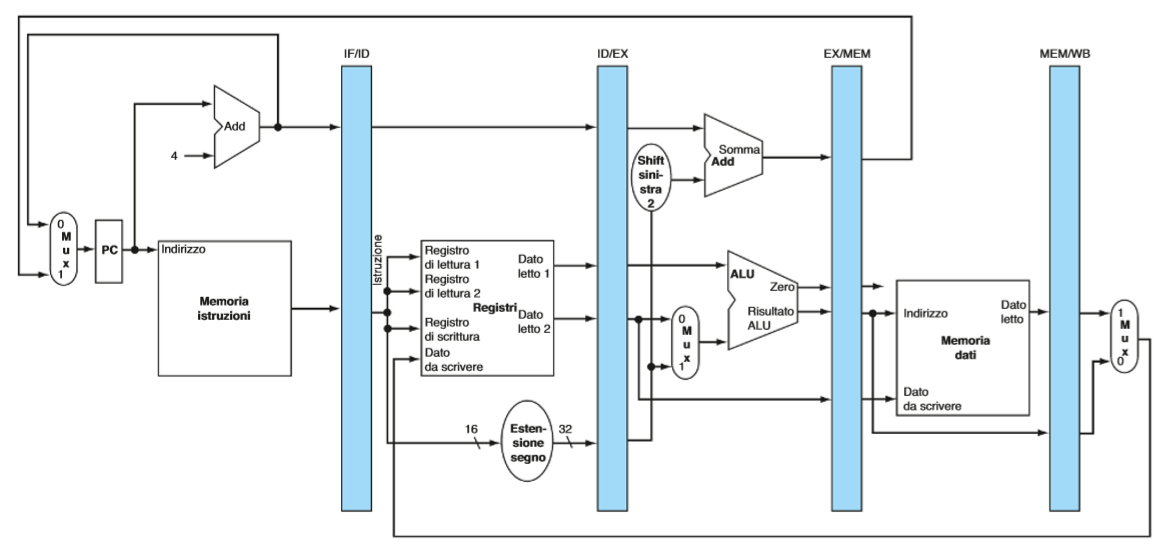
\includegraphics[width=\textwidth,keepaspectratio]{registri-di-backup.png}
\end{figure}
Un'altro aspetto interessante riguarda le dimensioni che questi registri devono avere, queste infatti sono molto variabili e dipendono strettamente da cosa il registro in causa deve memorizzare, il registro IF/ID, per esempio, deve essere ampio 64 bit, poiché deve contenere sia l’istruzione prelevata dalla memoria su 32 bit sia il contenuto del PC incrementato di 4, sempre su 32 bit. Gli altri tre registri di pipeline contengono rispettivamente 128, 97 e 64 bit.

\end{document}
